\section{Results \& Discussion}\label{sec:results}

\subsection{Fitting Sorption Parameters}\label{sec:results_sorption_fit}
% TODO: Make sure all your k_1 and k_2 descriptions are ok.
Figure \ref{fig:sorption_fit} shows the result of fitting the sorption data for three select materials - wood, Appling soil, and cinderblock concrete.
The $k_1$ and $k_2$ represent the rates at which TCE sorbs and desorbs respectively onto/from the material of interest.
The equilibrium partition constant, using the formulation in \eqref{eq:sorption_rate}, is given by
\begin{equation}
  K = \frac{k_1}{k_2}
\end{equation}
and defines the sorption isotherm.
Here a larger $K$ indicates that there is a greater propensity for contaminant sorption.\par

To apply a soil sorption isotherm in \eqref{eq:mass_transport} $K$ needs to be converted to $\mathrm{m^3/kg}$.
This is done by multiplying $K$ isotherm with inverse of the soil bulk density $\rho_b$, which is taken to be $1460 \; \mathrm{kg/m^3}$. % TODO: Cite the density
\begin{equation}
  K_\mathrm{ads} = \frac{K}{\rho_b} = 5.28 \; \mathrm{(m^3/kg)}
\end{equation}

\begin{figure}[htb!]
  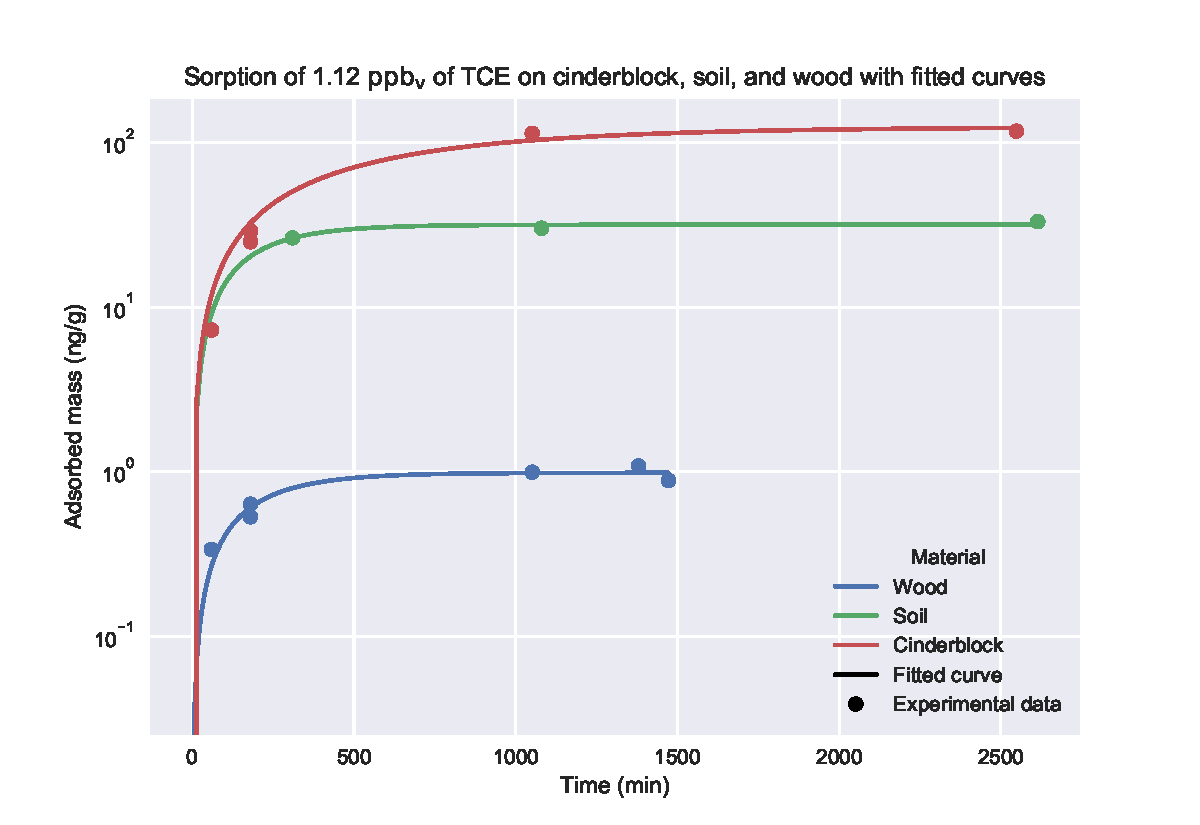
\includegraphics[width=\textwidth]{sorption_fit.pdf}
  \caption{Experimental data of sorption of TCE onto three select materials as well as fitted sorption rates based on the kinetic model \eqref{eq:sorption_rate}.}
  \label{fig:sorption_fit}
\end{figure}

Table \ref{tbl:sorption_fit} shows the fitted parameters for the tested materials.
Based on this these results we can see that cinderblock and soil have orders of magnitude larger sorption capacities than wood or drywall does.
We can also see by that soil and cinderblock sorb quickly, much faster than a material with similar sorptive capacity such as paper.\par

% TODO: Add the relative sorbed mass compared to air. I.e. cinderblock has ~ 7800 more mass for the same volume.
\begin{table}[htb!]
  \caption{Fitted kinetic sorption parameters based on sorption experiment data. Six different types of materials are considered. $k_1$ and $k_2$ are the sorption and desorption constants respectively, and $K$ is the sorption equilibrium constant.}
  \label{tbl:sorption_fit}
  \centering
  \begin{tabular}{l c c c}
    \toprule
    Material & $k_1 \; \mathrm{(1/hr)}$ & $k_2 \; \mathrm{(1/hr)}$ & $K$ \\
    \hline
    Wood & 44.90 & 0.32 & 140.90 \\
    Drywall & 87.94 & 0.41 & 214.87 \\
    Carpet & 58.74 & 0.26 & 226.21 \\
    Paper & 88.37 & 0.04 & 2195.69 \\
    Soil & 2636.57 & 0.34 & 7702.94 \\
    Cinderblock & 4175.16 & 0.10 & 41501.26 \\
    \bottomrule
  \end{tabular}
\end{table}

\subsection{Soil Sorption's Retarding Effect}\label{sec:retardation_effect}

The effect of building pressurization is a key factor in VI that influences the advective contaminant transport into or out of the building.
The magnitude of indoor contaminant concentration change in response to a pressurization change is significantly influenced by a variety of factors, such as soil permeability, foundation depth, soil moisture, and sorption.
To investigate the effect that soil sorption has on contaminant soil mass transport in the VI context, we have run two types transient simulation where initially the modeled structure is depressurized at a steady -5 Pa to establish a steady-state baseline.
At the start of the simulation, the building building is further depressurized to -15 Pa \eqref{eq:equilibrium_depressurization}, or overpressurized to 15 Pa \eqref{eq:equilibrium_overpressurization}, and the simulation is allowed to run for 72 hours. % TODO: Update this once the new simulations are done.
\begin{align}
  \text{Depressurization}: \; p_\mathrm{in} &= \begin{cases}
    -5, \; &t = 0 \; \mathrm{(hr)} \\
    -15, \; &0 < t \leq 72 \; \mathrm{(hr)}
\end{cases}\label{eq:equilibrium_depressurization}\\
\text{Overpressurzation}: \; p_\mathrm{in} &= \begin{cases}
  -5, \; &t = 0 \; \mathrm{(hr)} \\
  15, \; &0 < t \leq 72 \; \mathrm{(hr)}
\end{cases}\label{eq:equilibrium_overpressurization}
\end{align}
For each of these cases, the simulation is run using two different soil types - sand and sandy loam.
Sand is assumed here to not sorb any TCE, while for sandy loam a range of sorption isotherms are used.
These range from no sorption ($K_\mathrm{ads} = 0 \; \mathrm{(m^3/kg)}$) to the experimentally determined sorption isotherm for Appling soil ($K_\mathrm{ads} = 5.28 \; \mathrm{(m^3/kg)}$).
With the experimentally determined isotherm, we see that the ratio between sorbed concentration and soil-gas phase concentration is 7708, i.e. there is a much larger amount of contaminant sorbed to the soil than present in the vapor phase of the vadose zone.
When $K_\mathrm{ads} = 5.28 \cdot 10^{-4} \; \mathrm{(m^3/kg)}$ this ratio is roughly unity (0.77).\par

\begin{figure}[!htb]
  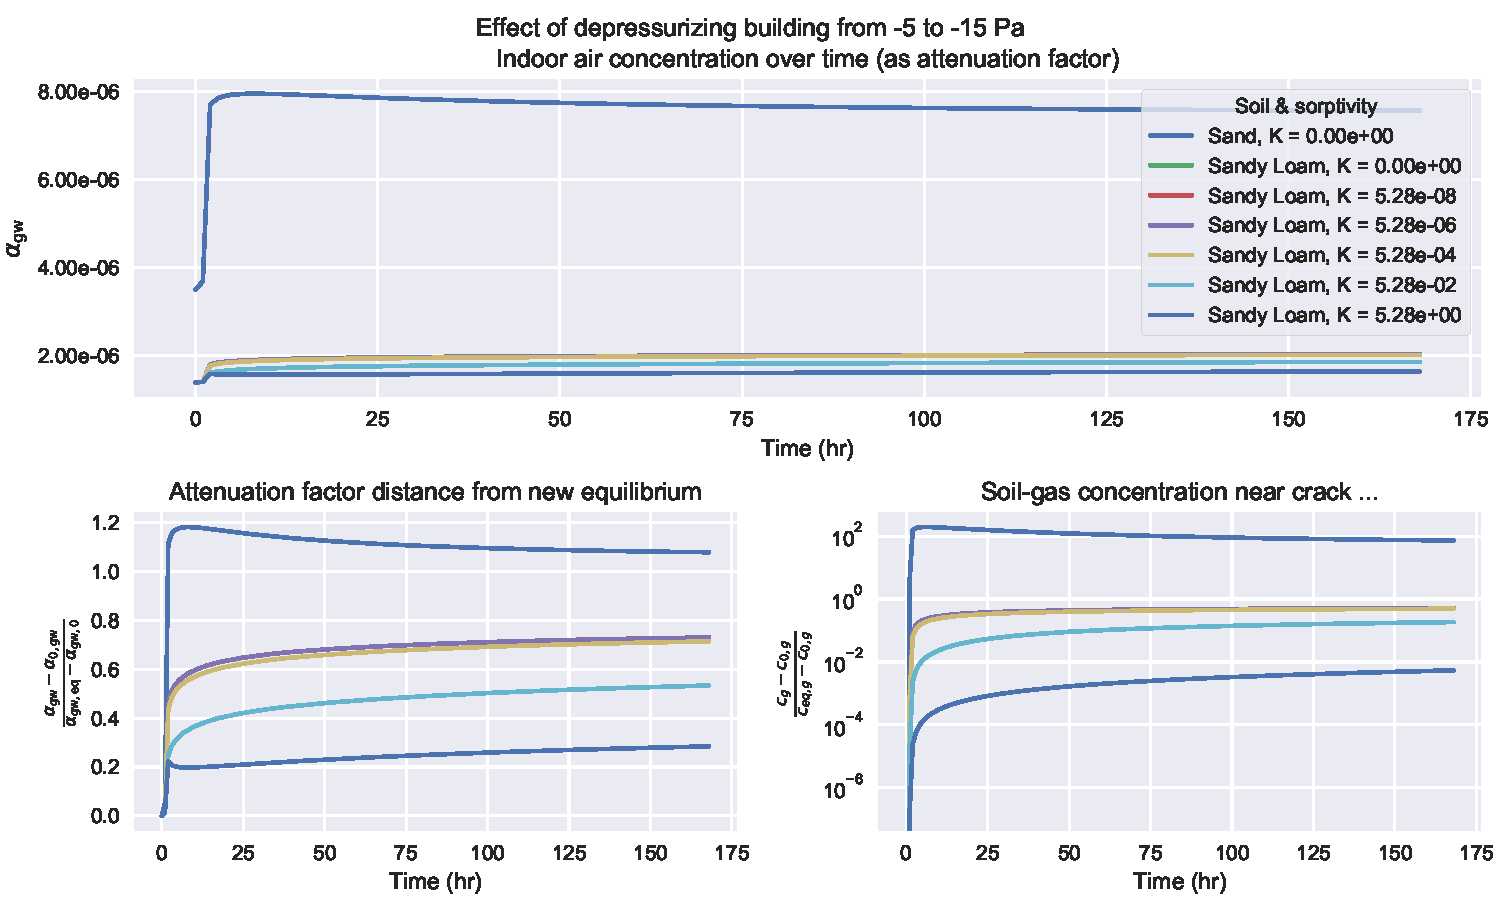
\includegraphics[width=\textwidth]{equilibrium_retardation_depressurization.pdf}
  \caption{}
  \label{fig:equilibrium_depressurization}
\end{figure}

The top panel of Figure \ref{fig:equilibrium_depressurization} shows the indoor air contaminant concentration as the simulated building is undergoing the depressurization as represented by the equation \eqref{eq:equilibrium_depressurization} case.
results are plotted as attenuation of contaminant relative to the groundwater source, i.e.
\begin{equation}
  \alpha = \frac{c_\mathrm{in}}{c_\mathrm{gw} K_H}
\end{equation}
Here we can see that when the surrounding soil consists of sand, the indoor concentration increases rapidly as the building is depressurized.
The increase is significantly smaller for the sandy loam cases, and becomes smaller as the sorbed mass increases ($K_\mathrm{ads}$ increases).\par

The bottom left panel shows the time for reaching the new equilibrium.
At the start of the simulation, the building starts at an attenuation of $\alpha_0$, which is the steady-state concentration when the building is depressurized to -5 Pa.
As the building is further depressurized to -15 Pa, the indoor air concentration will approach a new equilibrium state $\alpha_{eq}$ (the result of which is obtained from a steady-state simulation at that depressurization).
By plotting $\frac{|\alpha-\alpha_0|}{|\alpha_{eq}-\alpha_0|}$ we can see how far away we are from the new equilibrium state, and a value of 0 represents that we are at the initial concentration, i.e. $\alpha = \alpha_0$, and a value of 1 represents $\alpha = \alpha_{eq}$, i.e. that the new equilibrium has been reached.
This demonstrates that times of hundreds of hours may be needed to attain a near steady-state\par

The results of the same calculations are shown in the bottom right panel as well, but instead of plotting the indoor air concentration, we consider the average soil-gas concentration in a 5 cm diameter cylinder that envelops the entire perimeter crack.
The choice of 5 cm is arbitrary, but helps illustrate what happens in the near-foundation-crack region.
Examining these changes allow us to better understand how the contaminant is transported into the building from the soil.
Consistent with the long timescales for the indoor air to "adjust" to a new condition, the soil which is a significant source/sink for the contaminant share a similar slow adjustment.\par

Before discussing the role of sorption, we can first compare the non-sorbing sand and sandy loam cases.
Due to its higher permeability and lower moisture content, sand is significantly more permeable to gas flow than sandy loam (see Table \ref{tbl:model} for permeability values).
Consequently the advective transport through the foundation crack is much more significant in the sand case than the sandy loam case.
This may be characterized by a Péclet number for transport through the foundation crack, where
\begin{equation}\label{eq:peclet}
  \mathrm{Pe} = \frac{\mathrm{advection}}{\mathrm{diffusion}} = \frac{u_\mathrm{ck} L_\mathrm{slab}}{D_\mathrm{air}}
\end{equation}
and the Péclet number is around 4 versus 0.2 at a -15 Pa depressurization for sand and sandy loam respectively.
A Péclet greater than one indicate that advective transport dominates and vice versa.\par

Due to the advection dominated transport mechanism in the sand case, the indoor air concentrations are temporarily elevated above the final equilibrium concentration at -15 Pa.
(Note that the absolute distance from equilibrium is plotted in Figure \ref{fig:equilibrium_depressurization} which is why the concentration is two order of magnitude dispalced.)
This phenomena occurs because initially more contaminants are drawn into the building from the near crack area than can be resupplied, temporarily depleting the local soil-gas contaminant concentration.\par

One can notice that many of the sandy loam lines overlap, and start diverging from each other when $K_\mathrm{ads} = 5.28 \cdot 10^{-4} \; \mathrm{(m^3/kg)}$, at the point where the ratio of sorbed and soil-gas concentration are roughly equal.
Since the indoor air concentration depend on the soil-gas concentration, this is the origin of the difference.\par

The reason for this is that it is at this threshold the that sorptive contribution to the retardation factor \eqref{eq:retardation_factor} starts to becomes larger than the other terms.
\begin{equation}
   \rho_b K_H K_\mathrm{ads} > \theta_w + \theta_g K_H
\end{equation}
Thus it is at this point that the contaminant transport, i.e. replenishment from the source in the soil starts to become retarded by sorption.
The partitioning between the various phases controls residence time as the contaminant is transported.
Under VI conditions, the values of $\theta_w + \theta_g K_H$ are relatively small values, while $K_\mathrm{ads}$ can vary by orders of magnitude, making sorption potentially a very significant retarder for soil transport.\par

We can also note that the retarding effect of sorption also somewhat depends on the contaminants Henry's Law constant $K_H$, bulk density $\rho_b$ and the moisture content $\theta_w$.
For instance if the local temperature is higher, then contaminant $K_H$ is likewise larger, and the retardation factor is greater.
Generalizing this is difficult however, as $K_\mathrm{ads}$ decreases with temperature, and the interplay between these may be complicated.
Nevertheless this hints that there may be a climate/weather component to how significantly sorption induced retardation is.\par

Figure \ref{fig:equilibrium_overpressurization} shows the same sort of analysis as in Figure \ref{fig:equilibrium_depressurization} but with the building pressurization as described by \eqref{eq:equilibrium_overpressurization}.
As the building is overpressurized, the indoor contaminant is pushed back out into the soil.
Since the indoor air concentration is lower than the soil-gas concentration, a drop in local soil-gas concentration is observed along with a decrease in indoor air contaminant concentration.\par

\begin{figure}[!htb]
  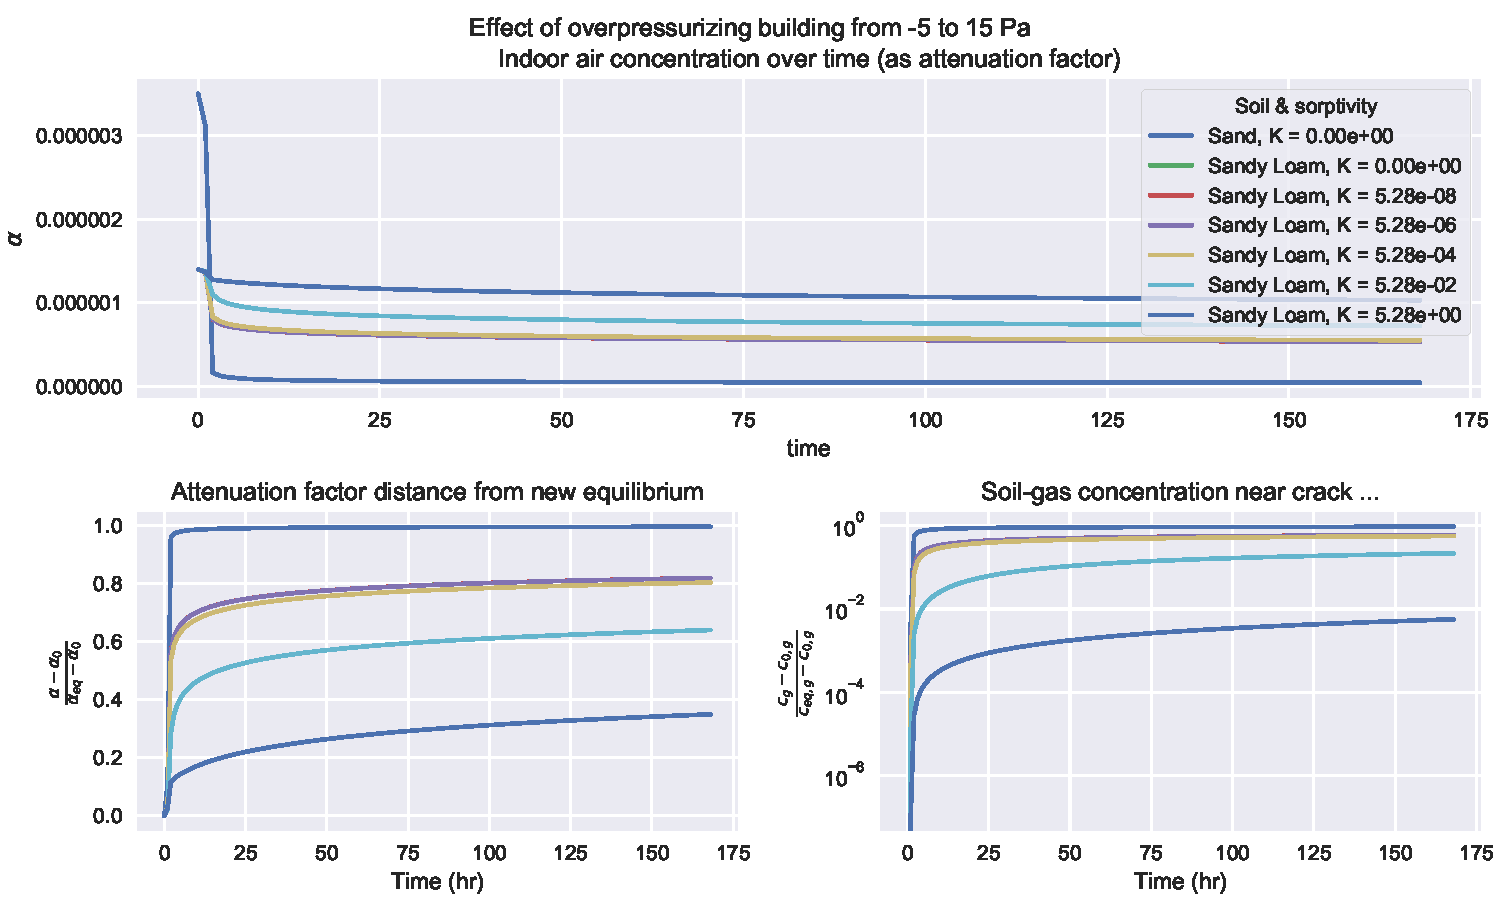
\includegraphics[width=\textwidth]{equilibrium_retardation_overpressurization.pdf}
  \caption{}
  \label{fig:equilibrium_overpressurization}
\end{figure}

% TODO: Some concluding remarks or keep this solely for the conclusion section?

\subsection{Effects of Indoor Material Sorption}\label{sec:results_indoor_sorption}

For these simulations we assume that there is no soil sorption.
We consider the basement (the indoor air space) and assume that the inside surfaces are entirely made up of one of the materials we presented in \ref{sec:results_sorption_fit}.
We also assume that the material covering the indoor surfaces has a certain thickness or depth that the contaminants can penetrate - providing a certain volume or mass of sorbing material in the indoor environment.
Table \ref{tbl:sorbed_material} shows the surface area, penetration depth, and volume of each material studied.
While the assumptions regarding coverage of different portions of the space are arbitrary, they are of the right order of magnitude and they do present some limiting cases of the potential effect of sorption onto/from these materials.\par

% TODO: Do I want to include some more information/data here? Sorbed mass at t0?
\begin{table}[htb!]
  \centering
  \begin{tabular}{l c c}
    \toprule
    Material & $d_\mathrm{p} \; \mathrm{(mm)}$ & $V_\mathrm{mat} \; \mathrm{(m^3)}$ \\
    \hline
    Cinderblock & 5 & 1.6 \\
    Wood & 1 & 0.32 \\
    Drywall & 10 & 3.2 \\
    Carpet & 10 & 3.2 \\
    Paper & 0.1 & 0.032 \\
    \bottomrule
  \end{tabular}
  \caption{The assumed contaminant penetration depth and subsequent volume of the sorbing indoor materials. The material surface area is assumed to be the same, and each material completely cover the surfaces of a 10x10x3 meter room.}
  \label{tbl:sorbed_material}
\end{table}

The modeled building then undergoes a pressurization cycle, in which at start of the simulation it has been depressurized at -5 Pa at steady-state.
The building is then sequentially depressurized to -15 Pa, then pressurized to 15 Pa, and finally again depressurized to -5 Pa.
For each sequence, the new pressurization is maintained for 24 hours.
This pressurization cycle may be seen in the top left panel of \ref{fig:indoor_sorption_cycle}.
The choice of pressurization cycle is somewhat arbitrary, but can be used to represent limiting cases of natural pressurization variation, or artificially induced pressurization.
Figure \ref{fig:indoor_sorption_cycle} shows the result of these simulations.\par

The change in indoor air contaminant concentration over this pressurization cycle is shown in the bottom panel of Figure \ref{fig:indoor_sorption_cycle}.
First we consider the reference case - where there is no sorbing indoor materials present.
(The blue line is the reference case, which may be difficult to see as the wood and carpet lines overlap.)
Here we see that as the building is depressurized, the indoor air contaminant concentration increases quickly in response to the depressurization change, and is approaching a new equilibrium.\par

% TODO: Plot the sorption rate r normalised to the entry rate n_ck? Should be ~1 when materials becomes saturated. Nice way to non-dimensionalize this too. Maybe as second axis plot on the top right panel?
\begin{figure}[!htb]
  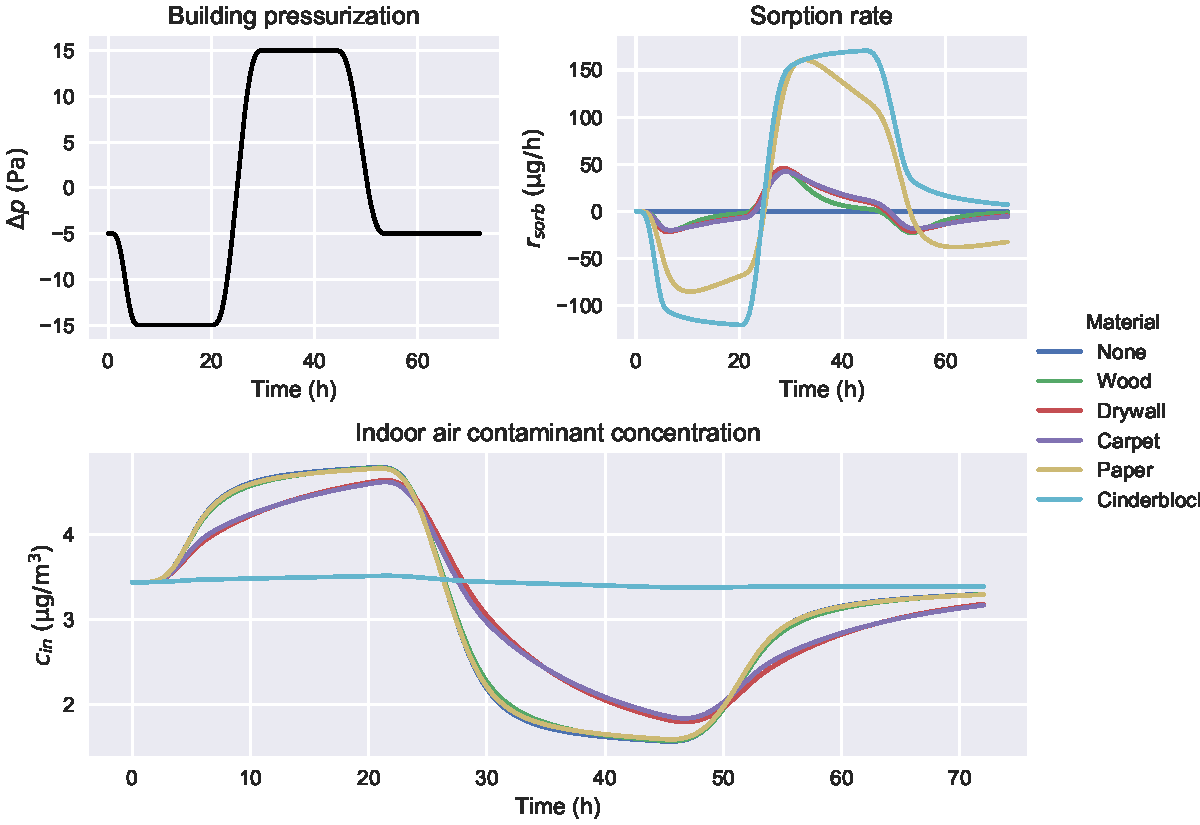
\includegraphics[width=\textwidth]{sorption_indoor_cycle.pdf}
  \caption{
  Comparison of how sorption onto/from various indoor materials affect the indoor air contaminant concentration (bottom) of a building that undergoes a pressurization cycle (top left). The rate of de- and sorption for each considered material during the cycle are also shown (top right) and is governed by \eqref{eq:sorption_rate}. A positive value means that contaminant vapors are being sorbed onto/into the material and a negative means the material is desorbing into the indoor air space.}
  \label{fig:indoor_sorption_cycle}
\end{figure}

The presence of the various studied building materials in the indoor environment have very different effects on the change in indoor air contaminant concentration.
The presence of wood and carpet has little effect on the indoor air concentration, whereas cinderblock has a very significant effect, dampening out almost any change in indoor concentration.
Drywall and carpet significantly delay the rate of change in the indoor concentration, but for each 24 hour cycle, roughly the same indoor concentration is reached as in the no sorbing material reference case.\par

The disparity in these result is explained by the the top right panel of Figure \ref{fig:indoor_sorption_cycle}.
Here the de- and sorption rates in $\mathrm{\mu g/hr}$ for each indoor material is shown.
A positive and negative value here indicate that contaminant is desorbed from or sorbed to the material respectively.
To understand this figure, it is useful to refer back to Table \ref{tbl:sorption_fit} which shows the sorption and desorption rate constant $k_1$ and $k_2$ respectively, and the sorption equilibrium constant $K$ (a larger value indicate a larger sorptive capacity).\par

First we consider to the depressurization part of the cycle (1-25 hours).
As in the indoor concentration panel, we see that the wood, drywall, and carpet cases overlap.
These materials have similar sorptive capacities ($K$) and sorptive rates ($k_2$).
Paper, by contrast, has a similar shape to the previous three but its magnitude is significantly larger.
This is because the $K$ value for paper is one order of magnitude larger, indicating that wood, drywall, and carpet saturate with contaminant vapors over the time period, while paper does not.
Cinderblock has a further order of magnitude larger $K$ value, thus is even further away from being saturated, which is consistent with its even faster sorption rate.\par

Next we consider the overpressurzation period (25-49 hours).
Again we see here that wood, drywall, and carpet behave the similarly.
This means that these reach the new contaminant saturation equilibrium at roughly the same time.\par

Here it is important to note that due to diffusion dominated transport through the foundation crack, even though the building is overpressurized, there is still substantial contaminant entry.
And because the sole contaminant source is contaminated groundwater, the sorbed equilibrium is determined by this entry rate.\par

Paper and cinderblock initially behave very similarly during the overpressurization period and desorb contaminants quickly.
However, paper reaches its saturation limit after a relatively short time, while cinderblock has not even at the end of the overpressurization cycle.
Since the desorption rate constants $k_2$ are relatively similar for the materials, this disparity is primarily due to the different sorption equilibrium constants $K$.\par

Lastly, we consider the final period where the pressurization goes back to its initial state (49-72 hrs).
Here we see that the reference case does not quite return to the initial indoor concentration.
Thus the contaminant entry rate has not equilibrated yet, because the soil contaminant concentration has not done so either.
As in the previous analysis we again see that the wood, drywall, and carpet cases don't differ from the reference.
Paper is slightly different, for the same reasons that have already been discussed.
Cinderblock is unique here, as it is releasing contaminants, due to the previous change in contaminant concentration.
In other words, it is acting as a significant capacitance in the system.\par

From this simulation work the varied the effects of sorbing indoor materials are apparent.
Most of the tested materials only have a moderate effect on the indoor air contaminant concentration dynamics, with the notable exception of cinderblock, which effectively maintains as pseudo-steady-state.
However we also see from the analysis of the sorption dynamics that the desorption and sorption rate constants $k_1$ and $k_2$ are less important than the overall sorptive capacity $K$ of the material.\par

\subsection{Indoor Material Sorption And Mitigation}\label{sec:results_indoor_mitigation}

The work done by us and others has shown the large sorptive capacities of various common materials.
The desorption of the sorbed contaminants may have significant impact on the apparent efficacy of various mitigation systems.
To investigate this we consider a scenario where initially the modeled building is depressurized at -5 Pa and at the start of the simulation some perfect mitigation scheme is implemented and the contaminant entry $n_\mathrm{entry}$ in \eqref{eq:cstr} goes to zero.
We also assume that for each case, the indoor environment contains the same amount of indoor material as described in section \ref{sec:results_indoor_sorption}.
The air exchange rate is assumed to remain a constant 0.5 per hour for the entire simulation time.\par

Hence, we can drop $n_\mathrm{ck}$ in \eqref{eq:cstr} and the equations used to model the indoor concentration becomes:
\begin{align}
  V_\mathrm{bldg} \frac{\partial c_\mathrm{in}}{\partial t} &= A_e c_\mathrm{in} V_\mathrm{bldg} - r_\mathrm{sorb} V_\mathrm{mat}\label{eq:cstr} \\
  V_\mathrm{mat} \frac{\partial c_\mathrm{sorb}}{\partial t} &= r_\mathrm{sorb} V_\mathrm{mat}\label{eq:sorbed_concentration} \\
  r_\mathrm{sorb} &= k_1 c_\mathrm{in} - k_2 c_\mathrm{sorb}\label{eq:sorption_rate}
\end{align}
This system of ordinary differential equations can be solved analytically.
A solution to this is
\begin{equation}
  \begin{bmatrix}
    c_\mathrm{in} \\ c_\mathrm{sorb}
  \end{bmatrix} =
  A \exp{(\lambda_1 t)} \vec{v_1} + B \exp{(\lambda_2 t)} \vec{v_2}
\end{equation}
and finding the eigenvalues ($\lambda_1, \; \lambda_2$) and eigenvectors ($\vec{v_1}, \; \vec{v_2}$) of the system above, allows us to calculate the indoor and sorbed contaminants concentrations through time.
$A$ and $B$ are constants found using the initial conditions
\begin{align}
  c_\mathrm{in}(t=0) = c_\mathrm{in,0} \rightarrow A \\
  c_\mathrm{sorb}(t=0) = c_\mathrm{sorb,0} K \rightarrow B
\end{align}
where we assume that $c_\mathrm{in,0} = 2 \; \mathrm{(\mu g/m^3)}$.\par

The decrease in indoor air concentration (as attenuation factor $\alpha$) for each case is seen in the top panel of Figure \ref{fig:sorption_mitigation}.
As expected, when there is no sorbing indoor materials, i.e. our reference case, the indoor concentration decreases log-linearily.
We can also see that contaminant desorption from materials maintains a higher indoor air concentration relative to reference, with cinderblock again shown to have the great impact.\par

\begin{figure}[!htb]
  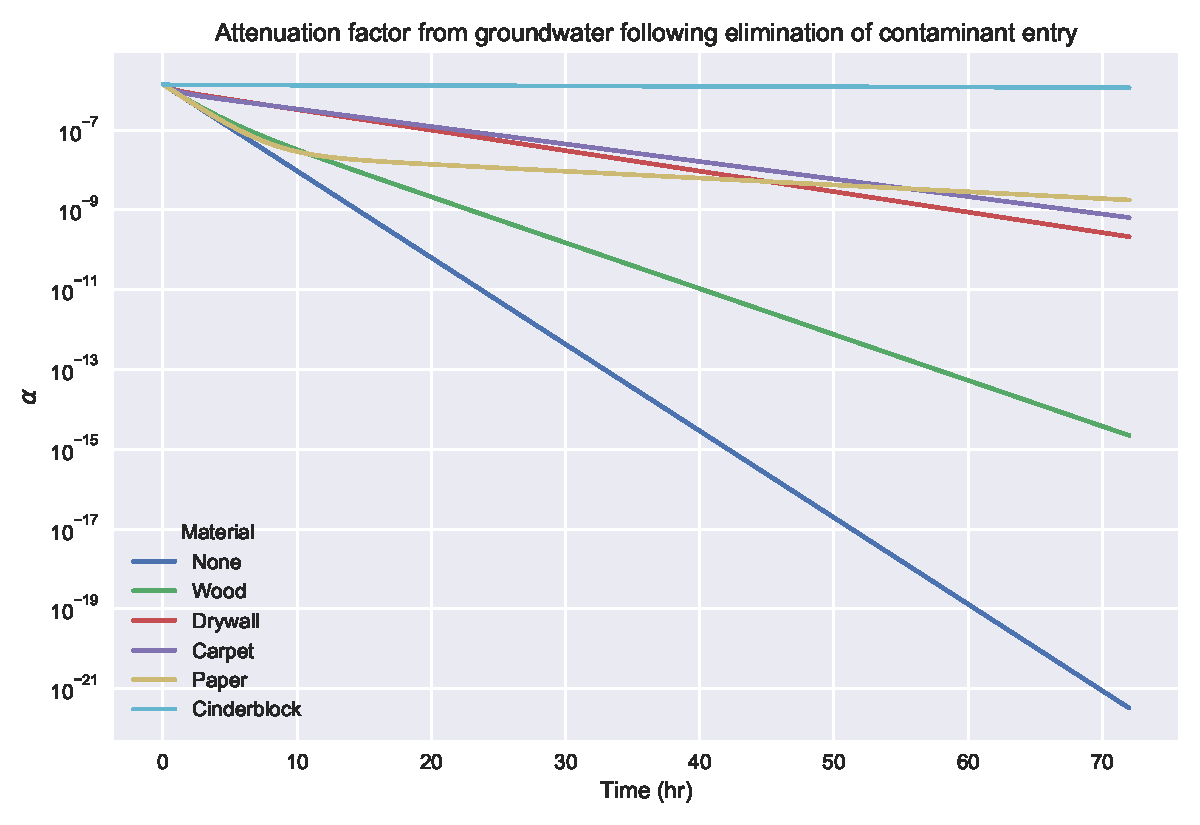
\includegraphics[width=\textwidth]{sorption_mitigation.pdf}
  \caption{Contaminant desorption from indoor materials delay the decrease in indoor contaminant concentration after a mitigation system has been implemented. The top panel shows the indoor air concentration after system implementation, considering desorption from different materials. The bottom panel quantifies how long it takes for the indoor concentration to decrease by a certain factor, considering the different cases.}
  \label{fig:sorption_mitigation}
\end{figure}

Clearly, the contaminant desorption from indoor materials can significantly delay the time that a certain reduction in indoor air concentration after a successful mitigation system has been implemented.
In the bottom panel of Figure \ref{fig:sorption_mitigation} we quantified the number of hours for a fifty percent, a one, and two orders of magnitude reduction in indoor air concentration to occurs, both absent sorbing indoor materials (the reference case) and in the presence of the one's presented earlier in this work.
On the x-axis the indoor air concentration reduction factor is shown, and on the y-axis the number of hours for the specified reduction occur is displayed, for each material.
The number of hours for each case are also shown at the top of each bar.\par

From this, we see that it takes 1.4 hours for the a 50\% reduction in indoor air concentration to occur for the reference, paper, and wood cases, while this time increases up to 305 hours in the cinderblock case.
This indicates the significant effect that sorption of TCE onto cinderblock can potentially have on the efficacy on a VI mitigation scheme, with the remaining materials having a relatively minor or moderate effect; a trend we have seen in other parts of this work.\par
